\documentclass[13pt]{article}
\usepackage{amsmath}
\usepackage{amssymb}
\usepackage{amsfonts}
\usepackage{nccmath}
\usepackage{cancel}
\usepackage{color}
\usepackage{xcolor}
\usepackage{graphicx}
\usepackage[margin=0.2in]{geometry}
\usepackage[utf8]{inputenc}
\thispagestyle{empty}
\begin{document}
\par\noindent
\begin{fleqn}[4em]

% No.1
\begin{align*}
\boxed{\begin{aligned}
  & \textbf{No. 1. } \text{ Diketahui }
    f(x) = \frac{1}{4} x^4 - \frac{2}{3} x^3 - \frac{1}{2} x^2 + 2x - 1 \\
  & \boxed{\begin{aligned}
    & f'(x) = \frac{1 \cdot 4}{4} x^3 - \frac{2 \cdot 3}{3} x^2 - \frac{1 \cdot 2}{2} x + 2 \\
    & f'(x) = \frac{1 \cdot \cancel{4}}{\cancel{4}} x^3 - \frac{2 \cdot \cancel{3}}{\cancel{3}} x^2 - \frac{1 \cdot \cancel{2}}{\cancel{2}} x + 2 \\
    & f'(x) = x^3 - 2x^2 - x + 2 \\
  \end{aligned}}\;~\;
  \boxed{\begin{aligned}[t]
    & f''(x) = 3x^2 - 4x - 1
  \end{aligned}} \\
  & \textbf{a.} \text{ Nilai } x \text{ yang memberikan titik kritis.} \\
  & \text{Titik kritis terdapat pada } f'(x) = 0 \text{ atau } f'(x) \text{ tidak terdefinisi.} \\
  & f'(x) \text{ terdefinisi untuk semua nilai } x \\
  & \text{Cek } f'(x) = 0 \\
  & f'(x) = x^3 - 2x^2 - x + 2 = 0 \\
  & x^3 - 2x^2 - x + 2 = 0 \\
  & (x - 2)(x + 1)(x - 1) = 0 \\
  & x = -1, x = 2, x = 1 \\
  & \boxed{\therefore \text{Nilai } x \text{ yang memberikan titik kritis adalah } \left\{-1, 2, 1\right\}} \\
  & \textbf{b.} \text{ Menentukan di mana } f(x) \text{ naik dan } f(x) \text{ turun.} \\
  & \boxed{\begin{aligned}
    & {\color{purple}(1)}\; f(x) \text{ naik jika } f'(x) > 0 \\
    & {\color{purple}(2)}\; x^3 - 2x^2 - x + 2 > 0 \\
    & {\color{purple}(3)}\; (x - 2)(x + 1)(x - 1) > 0 \\
    & {\color{purple}(4)}\; -1<x<1\text{ atau }x>2 \\
    & {\color{purple}(5)}\; \boxed{
      \therefore \text{Jadi, fungsi naik pada interval } (-1,\:1)\cup (2,\:\infty)
    }
  \end{aligned}}\;~\;
    \boxed{\begin{aligned}
    & {\color{purple}(1)}\; f(x) \text{ turun jika } f'(x) < 0 \\
    & {\color{purple}(2)}\; x^3 - 2x^2 - x + 2 < 0 \\
    & {\color{purple}(3)}\; (x - 2)(x + 1)(x - 1) < 0 \\
    & {\color{purple}(4)}\; x<-1\text{ atau }1<x<2 \\
    & {\color{purple}(5)}\; \boxed{
      \therefore \text{Jadi, fungsi turun pada interval } (-\infty,\:-1)\cup (1,\:2)
    }
    \end{aligned}} \\
  & \textbf{c.} \text{ Menentukan di mana } f(x) \text{ cekung ke atas } f(x) \text{ cekung ke bawah.} \\
  & \boxed{\begin{aligned}[t]
    & {\color{purple}(1)}\; f(x) \text{ cekung ke atas jika } f''(x) > 0 \\
    & {\color{purple}(2)}\; 3x^2\:-\:4x\:-\:1>\:0 \\
    & {\color{purple}(3)}\; 3\left(x-\frac{2}{3}\right)^2-\frac{7}{3}>0 \\
    & {\color{purple}(4)}\; \left(x-\frac{2}{3}\right)^2>\frac{7}{9} \\
    & {\color{purple}(5)}\; x<\frac{-\sqrt{7}+2}{3}\quad \mathrm{atau}\quad \:x>\frac{\sqrt{7}+2}{3} \\
    & {\color{purple}(6)}\; \boxed{
      \begin{aligned}[t]
        & \therefore \text{Jadi, fungsi cekung ke atas pada interval } \\
        & \:\left(-\infty \:,\:\frac{-\sqrt{7}+2}{3}\right)\cup \left(\frac{\sqrt{7}+2}{3},\:\infty \:\right)
      \end{aligned} 
    }
  \end{aligned}}\;~\;
  \boxed{\begin{aligned}[t]
    & {\color{purple}(1)}\; f(x) \text{ cekung ke bawah jika } f''(x) < 0 \\
    & {\color{purple}(2)}\; 3x^2\:-\:4x\:-\:1<\:0 \\
    & {\color{purple}(3)}\; 3\left(x-\frac{2}{3}\right)^2-\frac{7}{3}<0 \\
    & {\color{purple}(4)}\; \frac{3\left(x-\frac{2}{3}\right)^2}{3}<\frac{\frac{7}{3}}{3} \\
    & {\color{purple}(5)}\; -\sqrt{\frac{7}{9}}<x-\frac{2}{3}<\sqrt{\frac{7}{9}} \\
    & {\color{purple}(6)}\; \frac{-\sqrt{7}+2}{3}<x<\frac{\sqrt{7}+2}{3} \\
    & {\color{purple}(7)}\; \boxed{
      \begin{aligned}[t]
        & \therefore \text{Jadi, fungsi cekung ke bawah pada interval } \\
        & \left(\frac{-\sqrt{7}+2}{3},\:\frac{\sqrt{7}+2}{3}\right)
      \end{aligned} 
    }
  \end{aligned}} \\
  & \textbf{d.} \text{ Tentukan nilai minimum dan maksimum.} \\
  & \text{Terdapat nilai minimum dan maksimum pada titik kritis } f'(x) = 0 \\
  & \text{dari soal } \textbf{a} \text{ ditemukan titik kritis pada } x \in \left\{-1, 2, 1\right\} \\
  & f(-1) = -\frac{31}{12}\:~\:\,\text{\color{purple} (Minimum lokal)}\\
  & f(1)  = \frac{1}{12}\:~\:~\:~\:~\:\text{\color{purple} (Maksimum lokal)}\\
  & f(2)  = -\frac{1}{3}\:~\:~\:~\:\;\text{\color{purple} (Minimum lokal)}\\
  & \textbf{e.} \text{ Titik balik terdapat pada } \left(-1,\:-\frac{31}{12}\right),\:\left(1,\:\frac{1}{12}\right), \text{ dan } \:\left(2,\:-\frac{1}{3}\right)
  \\ & \textbf{by Ammar Faizi}
\end{aligned}}
\end{align*}

% No.2
\begin{align*}
\boxed{\begin{aligned}
  & \textbf{No. 2. } \text{ Mencari asimtot tegak pada fungsi } \\
  & \textbf{a. } f(x) = \frac{x^2 - x - 2}{x + 1} \\
  & \frac{x^2 - x - 2}{x + 1}
    = \frac{(x + 1)(x - 2)}{x + 1}
    = \frac{\cancel{(x + 1)}(x - 2)}{\cancel{x + 1}}
    = x - 2 \\
  & \therefore f(x) \text{ tidak memiliki asimtot tegak} \\ ~ \\
  & \textbf{b. } f(x) = \frac{x^2 - x - 2}{x + 2} \\
  & \frac{x^2 - x - 2}{x + 2} = x+\frac{-3x-2}{x+2} = x-3+\frac{4}{x+2} \\
  & \therefore \text{Terdapat asimtot tegak } x=-2
  \\ & \textbf{by Ammar Faizi}
\end{aligned}}
\end{align*}

% No.3
\begin{align*}
\boxed{\begin{aligned}
  & \textbf{No. 3. } \text{ Mencari asimtot datar pada fungsi } \\
  & \textbf{a. } f(x) = \frac{1}{x^2} - 1 \\
  & \therefore \text{Terdapat asimtot datar } y=-1 \\ ~ \\
  & \textbf{b. } f(x) = \frac{1}{x - 1} \\
  & \therefore \text{Terdapat asimtot datar } y=0
  \\ & \textbf{by Ammar Faizi}
\end{aligned}}
\end{align*}

% No.4
\begin{align*}
\boxed{\begin{aligned}
  & \textbf{No. 4. } \text{ Menggambarkan fungsi } \\
  & f(x)=x^{3}-12x^{2}+36x+10 \\
  & 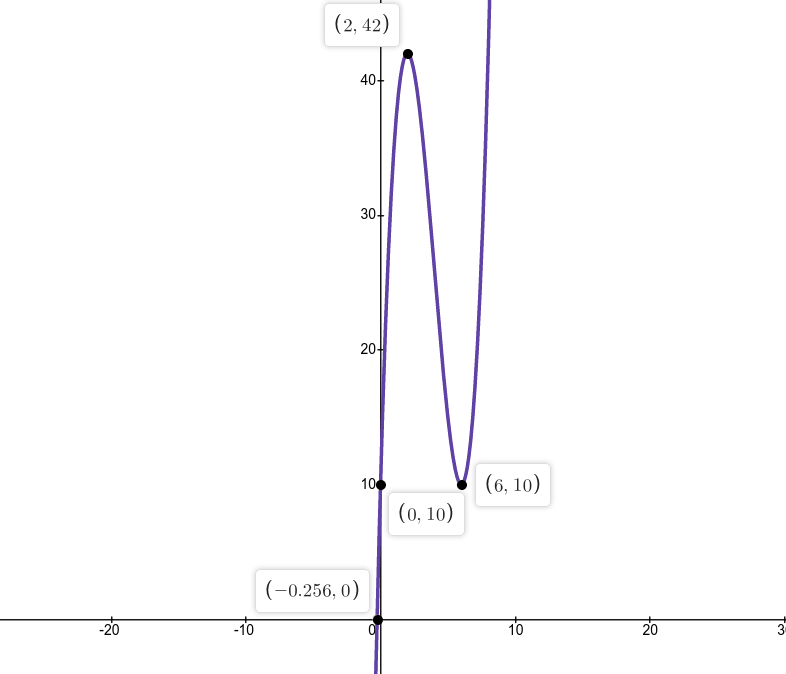
\includegraphics[scale=0.5]{graph_f.png}
\end{aligned}}
\end{align*}

% No.5
\begin{align*}
\boxed{\begin{aligned}
  & \textbf{No. 5. } \text{ Hitung limit } \\
  & \textbf{a. } \lim_{x \to -1} \frac{x^2 + 5x + 4}{x^2 - 4x -5}
    = \frac{(-1)^2 + 5(-1) + 4}{(-1)^2 - 4(-1) -5}
    = \frac{1 - 5 + 4}{1 + 4 -5}
    = \frac{0}{0} \text{ (bertemu dengan indeterminate form)} \\
  & \lim_{x \to -1} \frac{x^2 + 5x + 4}{x^2 - 4x -5}
    = \lim_{x \to -1} \frac{(x + 4)(x + 1)}{(x - 5)(x + 1)}
    = \lim_{x \to -1} \frac{(x + 4)\cancel{(x + 1)}}{(x - 5)\cancel{(x + 1)}}
    = \lim_{x \to -1} \frac{x + 4}{x - 5}
    = -\frac{3}{6} = -\frac{1}{2} \\ ~ \\ ~ \\
  & \textbf{b. } \lim_{x \to 1} \frac{\ln(x)}{x^2 - 1}
    = \frac{\ln(1)}{1^2 - 1}
    = \frac{0}{0} \text{ (bertemu dengan indeterminate form)} \\
  & \text{Menggunakan aturan L'Hopital} \\
  & \lim_{x \to a} \frac{f(x)}{g(x)} = \lim_{x \to a} \frac{f'(x)}{g'(x)} \\
  & \text{sehingga } \lim_{x \to 1} \frac{\ln(x)}{x^2 - 1}
    = \lim_{x \to 1} \frac{\frac{d}{dx} \ln(x)}{\frac{d}{dx}\left(x^2 - 1\right)}
    = \lim_{x \to 1} \frac{\frac{1}{x}}{2x}
    = \lim_{x \to 1} \frac{1}{2x^2}
    = \frac{1}{2} \\ ~ \\ ~ \\
  & \textbf{c. } \lim_{x \to \infty} \frac{x}{\ln(x)}
    = \frac{\infty}{\ln(\infty)}
    = \frac{\infty}{\infty} \text{ (bertemu dengan indeterminate form)} \\
  & \text{Menggunakan aturan L'Hopital} \\
  & \lim_{x \to a} \frac{f(x)}{g(x)} = \lim_{x \to a} \frac{f'(x)}{g'(x)} \\
  & \text{sehingga } \lim_{x \to \infty} \frac{x}{\ln(x)}
    = \lim_{x \to \infty} \frac{\frac{d}{dx}x}{\frac{d}{dx}\ln(x)}
    = \lim_{x \to \infty} \frac{1}{\frac{1}{x}}
    = \lim_{x \to \infty} x
    = \infty  \\ ~ \\ ~ \\
  & \textbf{d. } \lim_{x \to \infty} \frac{2x^2 + 5x + 4}{x^2 + 4x - 5}
    = \frac{\infty}{\infty} \text{ (bertemu dengan indeterminate form)} \\
  & \lim_{x \to \infty} \frac{2x^2 + 5x + 4}{x^2 + 4x - 5} \\
  &  = \lim_{x\to \infty}\frac{2+\frac{5}{x}+\frac{4}{x^2}}{1+\frac{4}{x}-\frac{5}{x^2}} \text{ (dibagi pangkat terbesar)} \\
  &  = \frac{2}{1} = 2
  \\ & \textbf{by Ammar Faizi}
\end{aligned}}
\end{align*}

\end{fleqn}
\end{document}
